\documentclass[10pt]{article}
\usepackage[utf8]{inputenc}
\usepackage[T1]{fontenc}
\usepackage{amsmath}
\usepackage{amsfonts}
\usepackage{amssymb}
\usepackage{mhchem}
\usepackage{stmaryrd}
\usepackage{graphicx}
\usepackage[export]{adjustbox}
\graphicspath{ {./images/} }
\usepackage{bbold}

\begin{document}
\section{Finite Element Method and Multigrid}
\subsection{A one dimensional problem}
8.1.1 Two-point boundary problems and finite element discretization

Define the functional space
$$
V=\{v:[0,1] \rightarrow R, v \text { is continuous and } v(0)=v(1)=0\} .
$$
Given any $f:[0,1] \rightarrow R$, consider
$$
J(v)=\frac{1}{2} \int_{0}^{1}\left|v^{\prime}\right|^{2} d x-\int_{0}^{1} f v d x .
$$
Find $u \in V$ such that
$$
u=\underset{v \in V}{\arg \min } J(v)
$$
Theorem 18. Problem (8.1) is equivalent to: Find $u \in V$ such that
$$
\left\{\begin{array}{l}
-u^{\prime \prime}=f, 0<x<1, \\
u(0)=u(1)=0 .
\end{array}\right.
$$
Proof. For any $v \in V, t \in R$, let $g(t)=J(u+t v)$. Since $u=$ $\arg \min _{v \in V} J(v)$ means $g(t) \geq g(0)$. Hence, for any $v \in V, 0$ is the global minimum of the function $g(t)$. Therefore $g^{\prime}(0)=0$ implies
$$
\int_{0}^{1} u^{\prime} v^{\prime} d x=\int_{0}^{1} f v d x \quad \forall v \in V
$$
By integration by parts, which is equivalent to
$$
\int_{0}^{1}\left(-u^{\prime \prime}-f\right) v d x=0 \quad \forall v \in V
$$
It can be proved that the above identity holds if and only if $-u^{\prime \prime}=f$ for all $x \in(0,1)$. Namely $u$ satisfies (8.10). $\square$ Let $V_{h}$ be finite element space and $\left\{\varphi_{1}, \varphi_{2}, \cdots \varphi_{n}\right\}$ be a nodal basis of the $V_{h}$ (see Section 5.2). Let $\left\{\psi_{1}, \psi_{2}, \cdots, \psi_{n}\right\}$ be a dual basis of $\left\{\varphi_{1}, \varphi_{2}, \cdots \varphi_{n}\right\}$, namely $\left(\varphi_{i}, \psi_{j}\right)=\delta_{i j}$.
$$
J\left(v_{h}\right)=\frac{1}{2} \int_{0}^{1}\left|v_{h}^{\prime}\right|^{2} d x-\int_{0}^{1} f v_{h} d x .
$$
Let
$$
v_{h}=\sum_{i=1}^{n} v_{i} \varphi_{i}
$$
then
$$
J\left(v_{h}\right)=I(v)=\frac{1}{2} v^{T} A * v-b^{T} v
$$
and
$$
\nabla I(v)=A * v-b .
$$
At the same time, let $u_{h}=\sum_{i=1}^{n} \mu_{i} \varphi_{i}$,
$$
u_{h}=\underset{v_{h} \in V_{h}}{\arg \min } J\left(v_{h}\right) \Leftrightarrow \mu=\underset{v \in R^{n}}{\arg \min } I(v)
$$
And $u_{h}$ solves the problem: Find $u_{h} \in V_{h}$
$$
\left.\frac{d}{d t} J\left(u_{h}+t v_{h}\right)\right|_{t=0}=a\left(u_{h}, v_{h}\right)-\left\langle f, v_{h}\right\rangle=0 \quad \forall v_{h} \in V_{h}
$$
where
$$
a\left(u_{h}, v_{h}\right)=\int_{0}^{1} u_{h}^{\prime} v_{h}^{\prime} d x
$$
which is equivalent to solving $\underline{A} \mu=b$, where $\underline{A}=\left(a_{i j}\right)_{i j}^{n}$ and $a_{i j}=$ $a\left(\varphi_{j}, \varphi_{i}\right)$ and $b_{i}=\int_{0}^{1} f \varphi_{i} d x .$ Namely
$$
\frac{1}{h}\left(\begin{array}{ccccc}
2 & -1 & & & \\
-1 & 2 & -1 & & \\
& \ddots & \ddots & \ddots & \\
& & -1 & 2 & -1 \\
& & & -1 & 2
\end{array}\right)\left(\begin{array}{c}
\mu_{1} \\
\mu_{2} \\
\vdots \\
\mu_{n}
\end{array}\right)=\left(\begin{array}{c}
b_{1} \\
b_{2} \\
\vdots \\
b_{n}
\end{array}\right) .
$$
Which can be rewritten as
$$
\frac{-\mu_{i-1}+2 \mu_{i}-\mu_{i+1}}{h}=b_{i}, \quad 1 \leq i \leq n, \quad \mu_{0}=\mu_{n+1}=0 .
$$
Using the convolution notation, (8.7) can be written as
$$
A * \mu=b
$$
where $A=\frac{1}{h}[-1,2,-1]$.

\subsubsection{Spectrum properties of $A *$}
We recall that $\lambda$ is an eigenvalue of $A$ and and $\xi \in R^{N} \backslash\{0\}$ is a corresponding eigenvector if
$$
A * \xi=\lambda \xi
$$
Because of the special structure of $A$, all the $N$ eigenvalues, $\lambda_{k}$, and the corresponding eigenvectors, $\xi^{k}=\left(\xi_{j}^{k}\right)$, of $A$ can be obtained, for $1 \leq k \leq N$, as follows:
$$
\lambda_{k}=\frac{4}{h} \sin ^{2} \frac{k \pi}{2(N+1)}, \quad \xi_{j}^{k}=\sin \frac{k j \pi}{N+1}(1 \leq j \leq N)
$$
Indeed, the relation $A \xi^{k}=\lambda_{k} \xi^{k}$ can be verified by following elementary trigonometric identities:

$-\sin \frac{k(j-1) \pi}{N+1}+2 \sin \frac{k j \pi}{N+1}-\sin \frac{k(j+1) \pi}{N+1}=4 \sin ^{2} \frac{k \pi}{2(N+1)} \sin \frac{k j \pi}{N+1}$,

where $1 \leq j \leq N$. Actually, it is not very difficult to derive these formula directly (see appendix A).

To understand the behavior of these eigenvectors, let us take $N=6$ and plot the linear interpolations of all these 6 eigenvectors. We immediately observe that each vector $\xi^{k}$ corresponds to a given frequency, and larger $k$ corresponds to higher frequency. As $\lambda_{k}$ is increasing with respect to $k$, we can then say that a larger eigenvalue of $A$ corresponds to a higher frequency eigenvector. From a numerical point of view, we say a relatively low frequency vector is relatively smoother whereas a high frequency vector is nonsmooth.

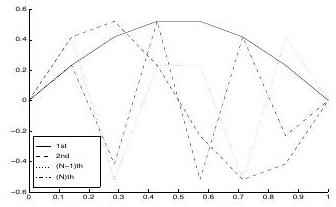
\includegraphics[max width=\textwidth]{2022_01_06_7eec630b8b060fb00b5bg-03}

Fig. 8.1. The eigenvectors We note that the set of eigenvectors $\xi^{k}=\left(\xi_{j}^{k}\right)$ forms an orthogonal basis of $R^{N}$. (This fact can be checked directly, or it also follows from the fact that the matrix $A$ is symmetric and has $N$ distinctive eigenvalues.) Therefore, any $\xi \in R^{N}$ can be expanded in terms of these eigenvectors:
$$
\xi=\sum_{k=1}^{N} \alpha_{k} \xi^{k}
$$
This type of expansion is often called discrete Fourier expansion. The smoothness of the vector $\xi$ has a lot to do with the relative size of the coefficients $\alpha_{k}$. To see this numerically, let us again take $N=4$ and consider the following two vectors
$$
\xi=\sum_{k=1}^{4} 2^{1-k} \xi^{k}, \quad \sigma=\sum_{k=1}^{4} 2^{k-4} \xi^{k}
$$
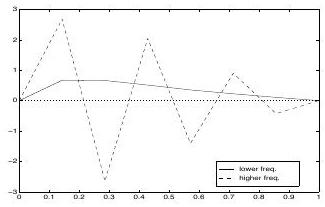
\includegraphics[max width=\textwidth]{2022_01_06_7eec630b8b060fb00b5bg-04}

Fig. 8.2. Plots of $\xi$ and $\sigma . \xi$-solid line; $\sigma$ dashed line

The first vector $\xi$ has larger coefficients in front of lower frequencies whereas the second vector $\sigma$ has larger coefficients in front of higher frequencies. From Figure $8.2$, it is easy to see how the smoothness of a vector depends on the relative size of its Fourier coefficients. We conclude that, in general, a vector with relatively small Fourier coefficients in front of the higher frequencies is relatively smooth and conversely, a vector with relatively large Fourier coefficients in front of the higher frequencies is relatively rough or nonsmooth.

\subsubsection{Gradient descent method}
Noting that $\nabla I(v)=A * v-b$ and applying the gradient descent method to solve problem (8.4), we obtain
$$
\mu^{(l)}=\mu^{(l-1)}-\eta\left(A * \mu^{(l-1)}-b\right), \quad l=1, \cdots, v .
$$
After $v$ iterations of gradient descent method, we denote the solution as $u_{h}^{\nu}$.

Consider the finite element discretization of Poisson equation in 1D: One very simple iterative method for (8.6) is the following gradient descent method
$$
\mu^{(l)}=\mu^{(l-1)}+\eta\left(b-A * \mu^{(l-1)}\right),
$$
or, for $j=1: N$,
$$
\mu_{j}^{(l)}=\mu_{j}^{(l-1)}+\eta\left(\beta_{j}-\frac{-\mu_{j-1}^{(l-1)}+2 \mu_{j}^{(l-1)}-\mu_{j+1}^{(l-1)}}{h}\right),
$$
where $\eta>0$ is a positive parameter named learning rate.

It is not so difficult to properly choose $\eta$ so that the above iterative scheme converges, namely for any initial guess $\mu^{0}$, the sequence $\left(\mu^{\prime} l-\right.$ 1)) generated by the above iteration converges to the exact solution $\mu$ of (8.6):

Note that
$$
\mu=\mu+\eta(b-A * \mu)
$$
we get
$$
\mu-\mu^{(l)}=(I-\eta A *)\left(\mu-\mu^{(l-1)}\right)
$$
Or
$$
\mu-\mu^{(l)}=(I-\eta A *)^{I}\left(\mu-\mu^{0}\right), l=1,2,3, \cdots
$$
As we known,
$$
(I-\eta A *)^{I} \longrightarrow o
$$
if and only if $\rho(I-\eta A *)<1$. Here $\rho(B)$ is the spectral radius of matrix $B$. However, $\rho(I-\eta A *)<1$ if and only if
$$
0<\text { all the eigenvalue of } A *<2 \eta^{-1} \text {. }
$$
Thus, a necessary and sufficient condition for the convergence is the following
$$
0<\eta<\frac{2}{\rho(A *)}
$$
It is easy to see that (for example, $4 / h$ is an upper bound of its row sums)
$$
\frac{4}{h}>\rho(A *)
$$
Therefore it is reasonable to make the following choice:
$$
\eta=\frac{h}{4}
$$
and the resulting algorithm is
$$
\mu^{(l)}=\mu^{(l-1)}+\frac{h}{4}\left(b-A * \mu^{(l-1)}\right)
$$
In the rest of this section, unless otherwise noted, we shall choose $\eta$ as above for simplicity.

On Figure $8.3$ the convergence history plot of the above gradient descent iterative method for typical application is shown. As we see, this iterative scheme converges very slowly.

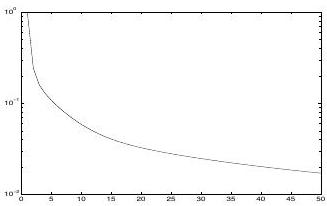
\includegraphics[max width=\textwidth]{2022_01_06_7eec630b8b060fb00b5bg-06}

Fig. 8.3. A picture on the GD method convergence history

Our main goal is to find a way to speed up such kind of rather slowly convergent iterative scheme. To do that, we need to study its convergent property in more microscopic level. First of all, let us now take a careful look at the convergence history picture and make the following observation:

Observation 1. The scheme converges rather fast in the very beginning but then slows down after a few steps. Overall, the method converges very slowly.

To further understand this phenomenon, let us plot the detailed pictures of the error functions in the first few iterations. After a careful look at these pictures, we have the following observation

Observation 2. The scheme not only converges fast in the first few steps, but also smooth out the error function very quickly.

In other words, the error function becomes a much smoother function after a few such simple iterations. This property of the itera-

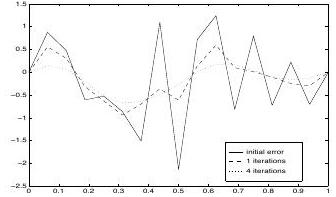
\includegraphics[max width=\textwidth]{2022_01_06_7eec630b8b060fb00b5bg-07}

Fig. 8.4. The smoothing effect of the Richardson method

tive scheme is naturally called a smoothing property and an iterative scheme having this smoothing property is called a smoother.

The above two observations, especially the second one, concern the most important property of the simple gradient descent method that we can take advantage to get a much faster algorithm.

Example 7. Let $f(x)=\pi^{2} \sin \pi x$. Consider
$$
\left\{\begin{array}{l}
-u^{\prime \prime}=f, 0<x<1, \\
u(0)=u(1)=0 .
\end{array}\right.
$$
The true solution $u=\sin \pi x$. Given the partition with the grid points $x_{i}=\frac{i}{n+1}, i=0,1, \cdots, n+1$, then by finite element discretization, we obtain
$$
A * \mu=b, A=\frac{1}{h}[-1,2,-1]
$$
Use gradient descent method to solve (8.11) with random initial guess $\mu^{0}$. Plot $\mu^{\ell}-\mu^{0}$ and $\left\|\mu^{\ell}-\mu^{0}\right\|$ for $\ell=1,2,3$.

The gradient descent method can be written in terms of $S_{0}^{\ell}: \mathbb{R}^{N_{t}} \rightarrow$ $\mathbb{R}^{N_{t}}$ satisfying
$$
\mu^{(1)}=\left(S_{0}^{\ell} b\right)=\frac{h_{\ell}}{4} b,
$$
for equation (8.7) with initial guess zero. If we apply this method twice, then
$$
\mu^{(2)}=S_{1}^{\ell}(b)=S_{0}^{\ell} b+S_{0}^{\ell}\left(b-A_{\ell} *\left(S_{0}^{\ell} b\right)\right),
$$
with element-wise form
$$
\mu_{i}^{(2)}=\frac{h_{\ell}}{16}\left(b_{i-1}+6 b_{i}+b_{i+1}\right)
$$
Then by the definition of convolution (6.17), we have
$$
\mu^{(1)}=S_{0}^{\ell} * b \quad \mu^{(2)}=S_{1}^{\ell} * b .
$$
with
$$
S_{0}^{\ell}=\frac{h_{\ell}}{4},
$$
and
$$
S_{1}^{\ell}=\frac{h_{\ell}}{16}[1,6,1]
$$
Hence we denote $S_{0}^{\ell}$ or $S_{1}^{\ell}$ as $S^{\ell}$.

Now for any given $\mu^{(0)}=\tilde{\mu}^{(0)}$,
$$
\begin{aligned}
&j=1,2, \cdots, 2 v \\
&\mu^{(j)}=\mu^{(j-1)}+S_{0}^{\ell} *\left(b-A * \mu^{(j-1)}\right) \\
&\Leftrightarrow \\
&j=1,2, \cdots, v \\
&\tilde{\mu}^{(j)}=\tilde{\mu}^{(j-1)}+S_{1}^{\ell} *\left(b-A * \tilde{\mu}^{(j-1)}\right)
\end{aligned}
$$
we obtain $\mu^{(j)}=\tilde{\mu}^{(j)}$ which means one step $S_{1}^{\ell}$ is equivalent to two steps of $S_{0}^{\ell}$.

\subsubsection{Convergence and smoothing properties of GD}
Because of the extraordinary importance of this smoothing property, we shall now try to give some simple theoretical analysis. To do this, we make use of the eigenvalues and eigenvectors of the matrix $A$.

\section{Fourier analysis for the gradient descent method}
Our earlier numerical experiments indicate that the gradient descent method has a smoothing property. Based on our understanding of the relation between the smoothness and the size of Fourier coefficients, we can imagine that this smoothing property can be analyzed using the discrete Fourier expansion.

Let $\mu$ be the exact solution of (8.6) and $\mu^{(l)}$ the result of $l-t h$ iteration from the gradient descent method (8.9). Then
$$
\mu-\mu^{(l)}=(1-\eta A *)\left(\mu-\mu^{(l-1)}\right)=\ldots=(1-\eta A *)^{l}\left(\mu-\mu^{(0)}\right) .
$$
Consider the Fourier expansion of the initial error:
$$
\mu-\mu^{(0)}=\sum_{k=1}^{N} \alpha_{k} \xi^{k}
$$
Then
$$
\mu-\mu^{(l)}=\sum_{k=1}^{N} \alpha_{k}(I-\eta A *)^{l} \xi^{k} .
$$
Note that $\eta=h / 4$ and for any polynomial $p$
$$
p(A *) \xi^{k}=p\left(\lambda_{k}\right) \xi^{k}
$$
we get
$$
\mu-\mu^{(m)}=\sum_{k=1}^{N} \alpha_{k}\left(1-\eta \lambda_{k}\right)^{m} \xi^{k}=\sum_{k=1}^{N} \alpha_{k}^{(m)} \xi^{k}
$$
where
$$
\alpha_{k}^{(m)}=\left(1-\sin ^{2} \frac{k \pi}{2(N+1)}\right)^{m} \alpha_{k} .
$$
Note that
$$
1-\sin ^{2} \frac{k \pi}{2(N+1)}=\cos ^{2} \frac{k \pi}{2(N+1)}=\sin ^{2}\left(\frac{\pi}{2}-\frac{k \pi}{2(N+1)}\right)
$$
implies
$$
\alpha_{k}^{(m)}=\alpha_{k} \sin ^{2 m} \frac{N+1-k}{N+1} \frac{\pi}{2} \leq \alpha_{k}\left(\frac{N+1-k}{N+1} \frac{\pi}{2}\right)^{2 m}
$$
which, for $k$ close to $N$, for example $k=N$, approaches to 0 very rapidly when $m \rightarrow \infty$. This means that high frequency components get damped very quickly. However, for $k$ far away from $N$, for example $k=1, \alpha_{k}^{(m)}$ approaches to 0 very slowly when $m \rightarrow \infty$.

This simple analysis clearly justifies the smoothing property that has been observed by numerical experiments.\\

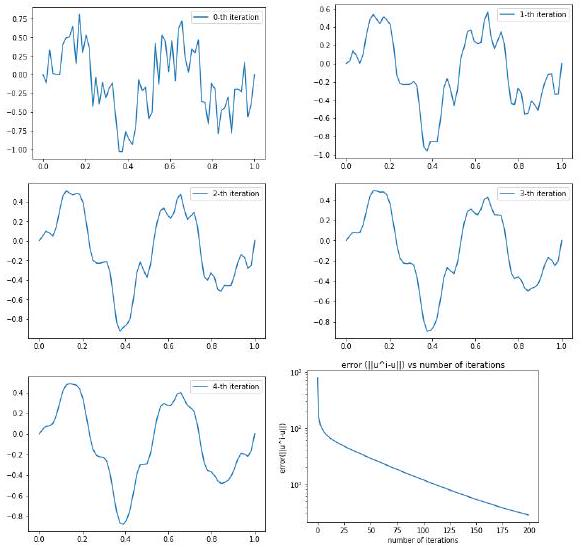
\includegraphics[max width=\textwidth]{2022_01_06_7eec630b8b060fb00b5bg-10}

Fig. 8.5. $u^{0}, u^{1}, u^{2}, u^{3}, u^{4}$ CHAPTER 8. FINITE ELEMENT METHOD AND MULTIGRID

METHOD IN CONVOLUTION

Jinchao $\mathrm{Xu}$

An intuitive discussion

Both the gradient decsent and Gauss-Seidel methods are oftentimes called local relaxation methods. This name refers to the fact that what both of these algorithms do are just trying to correct the residual vector locally at one nodal point at a time (recall that $\mu_{j} \approx u\left(x_{j}\right)$ ). This local relaxation procedure is then effective to the error components that are local in nature. Incidently, the nonsmooth or high frequency component which oscillates across one or few grid points have a strong local feature. Therefore, it is not surprising the both gradient descent and Gauss-Seidel iteration can damp out these nonsmooth components more easily. These methods are very inefficient for relatively smoother components in the error since a smoother function is more globally related in nature.


\end{document}